To obtain an insight into the power consumption with the introduction of the config NoC changes in \cref{TODO} and model configuration using external memory we will provide an comprehensive analysis.
% To get an approximation of the power consumption when configuring the GrAICore with a model and processing frames with it, we will provide calculations with energy parameters acquired from internal sources.

When configuring the GrAICore and processing an input frame, the major components that consume energy are as follows:
\begin{itemize}
    \item Configuration
    \begin{itemize}
        \item Reading data from the external memory
        \item Transferring data from the external memory to the config NoC
        \item Phits traversing (i.e., hops) through the config NoC
        \item Writing data to the neuron core's SRAM
    \end{itemize}
    \item Processing
    \begin{itemize}
        \item Processing the input frame by the model
    \end{itemize}
\end{itemize}

\section{Configuration energy}
Since we have access to various energy parameters for DDR memory, we will use DDR memory as an example.

\begin{figure}[hbtp]
    \centering
    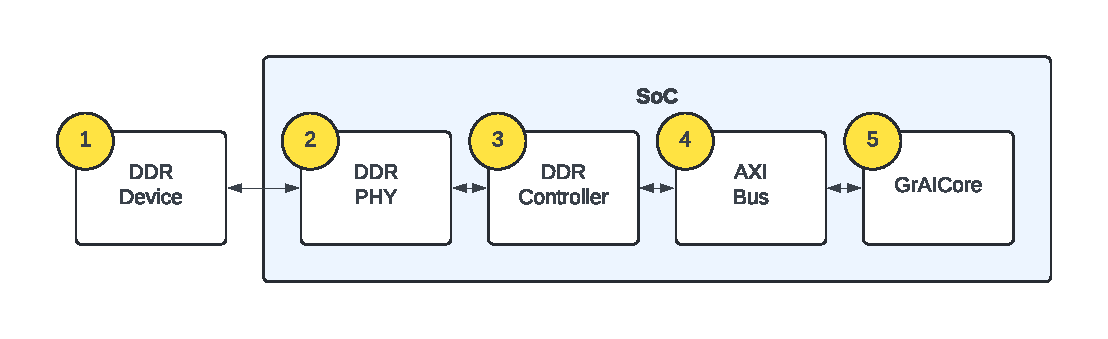
\includegraphics[width=0.8\linewidth]{assets/ddr_graicore_block_diagram.pdf}
    \caption{
        Interconnection of the DDR device and GrAICore
    }
    \label{fig:ddr_graicore_block_diagram}
\end{figure}

A typical system with DDR as external memory looks as shown in \cref{fig:ddr_graicore_block_diagram}.
% TODO add image
\begin{itemize}
    \item The \textit{DDR device} where the (model) data is read from.
    \item The \textit{DDR PHY} that connects the \textit{DDR device} and \textit{DDR controller}.
    \item The \textit{DDR controller} that handles the read/write requests from the \textit{GrAICore}.
    \item The \textit{AXI bus} that connects the \textit{DDR controller} and \textit{GrAICore}.
    \item The \textit{GrAICore} that transfers and writes data the SRAMs.
\end{itemize}

% It has been established that performing a hop on the Event NoC consumes around \SI{129}{fJ}.
% These hops are for phits of 32 bits.
% For the Config NoC (which uses phits of 16 bits), we are interested in the energy use for transferring phits of 16 bits. We can approximate this value by dividing the value for 32 phit hops into two. I.e., 129 fJ / 2 = 64.5 fJ. 

% Furthermore, it has been established that for the SRAM to write 64 bits, it consumes \SI{2.490}{pJ}.
% The SRAM system has the property to write 64 bits at once by first buffering four consecutive phits.
% This improves efficiency. 

For the analysis, we assume that we are using the newly proposed config NoC in \cref{sec:proposed_noc}. 
With the new packet format, a packet contains at most 65 data phits of 64 bits each.
That is, a maximum of 520 bytes\footnote{$65 \times \frac{\SI{64}{b}}{8} = \SI{520}{B}$} of payload per packet.
Furthermore, an additional injection point is introduced (see \cref{fig:segmentation_example_2}).
Next to the injection point connected to the router on the bottom left of the config NoC, a new one is added and connected to the router six positions up.

To estimate the energy cost for configuration, we require the following information from a model:
\begin{itemize}
    % \item Amount of data to read from the external memory
    \item Amount of data to transfer to the SRAMs
    \item Core destination of the data
\end{itemize}

The amount of data to transfer determines how much data will be read, transferred and written.
We are assuming that the same amount of data read from the external memory is written to the SRAMs.
The location (specific neuron core) of the data determines the amount of hops the data has to perform in the config NoC.
The amount of data to write can also be used to determine the configuration time.
The configuration time is calculated by dividing the amount of data with the write bandwidth.
The configuration time is used for computing the energy for the \textit{DDR PHY}, \textit{DDR controller} and \textit{AXI bus}.

The amount of data to be written and to which neuron cores depends on how the compiler has performed the mapping on the GrAICore. % explain
Phits that needs to be transferred to neuron cores further away from an injection point will require more hops to reach, and therefore consume more energy than neuron cores closer to an injection point.
The amount of data that needs to be written to each core differs.
We can retrieve this information from the compiler.

For estimating the energy for the GrAICore component, we consider the config NoC and the SRAMs.
The config NoC consumes energy by transferring the phits to its destinations via one or multiple hops through the NoC.
The SRAM consumes energy by writing the data to its banks.
A single hop through the config NoC with a 64 bit phit consumes \SI{0.258}{pJ}.
Writing back 64 bits to an SRAM consumes \SI{4.980}{pJ}.

\begin{table}[hbtp]
\centering
\begin{tabular}{@{}lll@{}}
\toprule
\textbf{Component}      & \textbf{Usage}  &  \\
\midrule
DDR device              & \SI{0.11}{nJ/B} &  \\
DDR PHY                 & \SI{133}{mW}    &  \\
DDR controller          & \SI{20}{mW}     &  \\
AXI bus                 & \SI{80}{mW}     &  \\
NoC hop (\SI{64}{b})    & \SI{0.258}{pJ}  &  \\
SRAM write (\SI{64}{b}) & \SI{4.980}{pJ}  &  \\
\bottomrule
\end{tabular}
\caption{Energy parameters for each of the major energy consuming components. The shown power numbers for \textit{DDR PHY}, \textit{DDR controller} and \textit{AXI bus} are when at full capacity (i.e., best-case scenario).}
\label{tab:energy_parameters_ddr}
\end{table}

\subsection{Calculation}
The configuration energy consists of the reading, transferring and writing of data from the external memory to the GrAICore's SRAMs. 

Let $C$ be the set of tuples holding the coordinates of every core:
\begin{equation*}
    C = \{\,\left(x,y\right) \in \mathbb{N}^2 \mid 1 \leq x \leq 12 \wedge 0 \leq y \leq 11 \,\} 
\end{equation*}

Notice that the x-coordinate and y-coordinate starts at index $1$ and $0$ respectively.

\Cref{fig:model_data_heapmap} shows for a $80\%$ pruned version of ResNet-50\footnote{Internally named \texttt{resnet50\_pruned80\_star}} the amount of data that needs to be written to each of the 144 neuron cores.
We observe that the data is not uniformly distributed across the SRAMs.
Therefore, we require information how much data needs to be transferred to each SRAM.

\begin{figure}[hbtp]
    \centering
    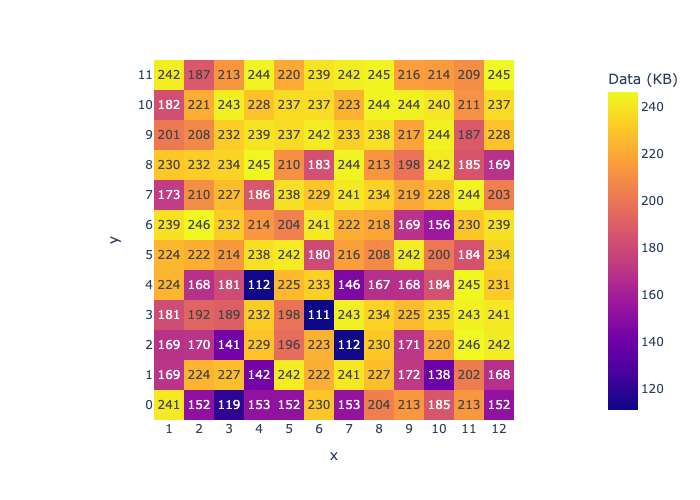
\includegraphics[width=0.8\linewidth]{assets/model_data_heatmap.png}
    \caption{Amount of data to be written to each core for the ResNet-50 model (80\% pruned).}
    \label{fig:model_data_heapmap}
\end{figure}

Let $D$ be a matrix of $12 \times 13$ with $D_{i,j}$ denoting the amount of bytes to be written to core $\left( i,j \right)$.
$D$ has an additional column due to the x-coordinates not starting from index $0$.
Its left-most column is unused (i.e., $D_{0,0}, D_{0,1}, \cdots, D_{0,11}$).
This matrix can be constructed from the artifacts outputted by the compiler.

The number of phits to be transferred through the config NoC influences the total energy costs.
In particular, the amount of phits to be transferred affects the number of hops to be taken in total and the amount of data to be written to the SRAMs.
Therefore, we need to determine how many phits needs to be transferred to each neuron core.
% The number of phits to be transferred influences the energy cost in the config NoC hops and SRAM writes.
% A packet can contain up to 520 bytes\footnote{$65 \times \frac{64}{8}$} of payload data. 
A packet can contain up to 65 data phits, that is $65 \times \SI{64}{b} = \SI{520}{B}$ of payload data.
% If we transfe
Suppose we need to transfer $d$ bytes to a neuron core, we then require a total of $\left\lfloor \frac{d}{520} \right\rfloor$ packets with 65 data phits.
% If $d \bmod 520 > 0$, then there is an additional packet consisting of $\left\lceil \frac{\left( d \bmod 520 \right) \times 8}{64}\right\rceil$ data phits.
If $\left( d \bmod 520 \right) > 0$, then there is an additional packet for the remaining $\left( d \bmod 520 \right)$ bytes of data.
The remaining packet will consist of $\left\lceil \frac{d \bmod 520}{8}\right\rceil$ data phits.
Note that each packet also contains a single phit of 64 bits for the header information.

The total energy cost for configuring the GrAICore can be estimated with the following equation:
\begin{equation}
    E_{\textrm{config}} = E_{\textrm{ext\_mem}} + E_{\textrm{noc}} + E_{\textrm{write}}
\end{equation}

With:
\begin{align*} 
E_{\textrm{ext\_mem}} &= 
        \sum_{c \in C}^{}{E_\textrm{read\_ext\_mem}(D_c) + E_{\textrm{send\_to\_noc}}(D_c)} \\
E_{\textrm{noc}} &=
    E_{\textrm{hop}} \times \sum_{c \in C}^{}{N_\textrm{hops}(c) \times p_{\textrm{total}}(D_c)} \\
E_{\textrm{write}} &=
    E_{\textrm{sram\_write\_64b}} \times \sum_{c \in C}^{}{p_{\textrm{data}}(D_c)}
\end{align*}

And:
\begin{align*} 
N_{\textrm{hops}}(x,y) &=
    \begin{cases} 
        x + y & \textrm{if } 0 \leq y \leq 5 \\
        x + y - 6 & \text{if } 6 \leq y \leq 11
    \end{cases}
\\
p_{\textrm{total}}(d) &=
    \left\lfloor \frac{d}{520} \right\rfloor \times (65 + 1) + \left\lceil \frac{d \bmod 520}{8} \right\rceil + 1 =
    \left\lceil \frac{d}{8} \right\rceil + \left\lfloor \frac{d}{520} \right\rfloor + 1 
\\
p_{\textrm{data}}(d) &=
    \left\lfloor \frac{d}{520} \right\rfloor \times 65 + \left\lceil \frac{d \bmod 520}{8} \right\rceil =
    \left\lceil \frac{d}{8} \right\rceil
\end{align*}

\begin{eqexpl}[15mm]
    \item{$p_{\textrm{total}}(D_c)$} total phits (includes headers) for transferring $D_c$ bytes
    \item{$p_{\textrm{data}}(D_c)$} total data phits (excludes headers) for transferring $D_c$ bytes
    \item{$N_{\textrm{hops}}(c)$} the amount of hops required to reach a neuron core at coordinate $c$, starting from the router closest to the injection point. It has two sub-functions due to the new config NoC's dual injector architecture
    \item{$E_{\textrm{read\_ext\_mem}}(D_c)$} energy for reading $D_c$ bytes from the external memory
    \item{$E_{\textrm{send\_to\_noc}}(D_c)$} energy for sending $D_c$ bytes from the external memory to the config NoC
    \item{$E_{\textrm{hop}}$} energy for performing a single hop in the config NoC
    \item{$E_{\textrm{sram\_write\_64b}}$} energy for writing back 64 bits to a neuron core's SRAM
\end{eqexpl}

\section{Processing energy}
The processing energy is the energy consumed when the GrAICore is processing input frames.
% Note that the GrAICore does not make use of the config NoC to process input frames.
Note that the GrAICore uses the event NoC for communication between nodes when processing input frames, the config NoC is not involved in this process.

The processing energy can be estimated with the following equation:
\begin{equation}
    E_{\textrm{frame}} = \textrm{avg\_util} \times \textrm{cores\_used} \times \textrm{processing\_latency} \times \SI{21}{mW}
\end{equation}

These parameters can be obtained by simulating the model with \textit{GrAIPEFRUIT}, an in-house simulator for estimating inference performance.
Processing latency (\textrm{processing\_latency}) is the time the model takes to fully process a single frame, from input to output.
Cores used (\textrm{cores\_used}) is the amount of neuron cores that were used to execute the model.
Average utilization (\textrm{avg\_util}) is the average percentage of the time the cores were active while the frame was processed. 
The constant \SI{21}{mW} is the approximated power usage of a single neuron core while it's being fully utilized.
This constant is obtained from internal RTL simulations.

Since the config NoC is not involved in the processing of an input frame, any change to the config NoC does not influence the processing energy.
A significant factor (other than hardware changes) that may affect the processing energy is the mapping performed by the compiler on the original model. 
Different mappings on the same model have an effect on the average utilization and the number of neuron cores used, which in turn influences the processing latency.

\section{Evaluation}
To develop a preliminary understanding of the power contributions of the model reconfiguration from external memory, we evaluate a variety of practical models.
The power is the configuration of a model and a single inference with the model at \SI{60}{FPS}.
Effectively, this means that the same model is configured on the GrAICore 60 times per second and also used to proces an input frame 30 times per second.

We will be looking at two different external memory technologies, LPDDR5X and PCM.
We assume we use the DDR protocol for transferring data to the AXI bus that is connected to the GrAICore.
For the DDR protocol to work, we require an DDR PHY and DDR controller.
These components both add to the energy when transferring data to the GrAICore.

\begin{table}[hbtp]
    \centering
    \begin{tabular}{@{}lrl@{}}
    \toprule
    \textbf{Component} & \textbf{Value} & \textbf{Unit} \\
    \midrule
    LPDDR5X read             & 36.00 & pJ/B \\
    PCM read                 & 5.29 & pJ/B  \\
    DDR PHY                  & 10.39 & pJ/B \\
    DDR Controller           & 1.56 & pJ/B  \\
    AXI Bus                  & 6.25 & pJ/B  \\
    Config NoC hop (64 bits) & 0.26 & pJ    \\
    SRAM write (64 bits)     & 4.98 & pJ    \\ \bottomrule
    \end{tabular}
    \caption{Energy parameters of PCM and LPDDR5X memory, DDR interface and GrAICore that are relevant for model configuration}
    \label{tab:energy_parameters}
\end{table}

We look at the models as shown in \cref{tab:example_models_stats}.
It also shows the processing latency, the number of cores used and the average utilization of the cores of each (mapped) model.
These statistics are used for computing the processing energy.
The ``to write'' columns show the total amount of bytes that is to be transferred to the GrAICore.
Note that to get a more accurate energy number for configuration, we need the amount of bytes to be transferred to each core individually.
This information is available, and will be used for the evaluation.

\begin{table}[]
\centering
\begin{tabular}{@{}lrrrrr@{}}
\toprule
\textbf{Model}          & \textbf{\begin{tabular}[c]{@{}l@{}}Latency\\ (ms)\end{tabular}} & \textbf{Cores} & \textbf{Avg util.} & \textbf{\begin{tabular}[c]{@{}l@{}}To write\\ (MiB)\end{tabular}} \\ \midrule
efficientnet            & 1.642                                                           & 144            & 50.89\%            & 16.15                                                             \\
mobnetv2                & 1.296                                                           & 144            & 40.78\%            & 10.67                                                             \\
hand\_tracker           & 1.480                                                           & 144            & 36.62\%            & 12.33                                                             \\
hand\_detector          & 4.809                                                           & 144            & 68.03\%            & 19.12                                                             \\
resnet50                & 5.765                                                           & 144            & 36.35\%            & 29.58                                                             \\
resnet101\_p0           & 7.080                                                           & 144            & 33.40\%            & 28.75                                                             \\
resnet101\_p1           & 2.647                                                           & 143            & 36.42\%            & 20.06                                                             \\
resnet101\_p2           & 4.011                                                           & 144            & 33.12\%            & 30.44                                                             \\
resnet101\_p3           & 2.343                                                           & 143            & 33.55\%            & 17.71                                                             \\
resnet101\_p4           & 2.040                                                           & 143            & 26.19\%            & 15.54                                                             \\
resnet101\_pruned\_p0   & 6.552                                                           & 144            & 38.10\%            & 15.87                                                             \\
resnet101\_pruned\_p1   & 3.245                                                           & 143            & 34.31\%            & 10.43                                                             \\
resnet101\_pruned\_p2   & 4.501                                                           & 143            & 33.83\%            & 16.00                                                             \\
resnet101\_pruned\_p3   & 2.114                                                           & 143            & 38.08\%            & 10.22                                                             \\
resnet101\_pruned\_p4   & 2.437                                                           & 143            & 24.25\%            & 7.69                                                              \\
\bottomrule
\end{tabular}
\caption{Model statistics}
\label{tab:example_models_stats}
\end{table}

As an example, we demonstrate a calculation for the ResNet-50 model.
The processing energy is calculated as follows:
\begin{equation}
    E_\textrm{proc} = 0.3635 \times 144 \times \SI{5.765}{ms} \times \SI{21}{mW} = \SI{6.34}{mJ}
\end{equation}

\Cref{fig:model_data_heapmap} shows for the mapped ResNet-50 the amount of data to be sent to each individual core.
We use this information to construct matrix $D$ and the configuration energy $E_\textrm{conf}$.
We obtain the values as shown in \cref{tab:resnet50_energy}.
Configuration with LPDDR5X of the ResNet-50 model on the GrAICore consumes \SI{1.71}{mJ} and with PCM \SI{0.76}{mJ}.

\begin{table}[hbtp]
    \centering
    \begin{tabular}{@{}ll@{}}
    \toprule
    \textbf{Component} & \textbf{Value} \\
    \midrule
    $\ereadlpddr5x$ & 1116.8 \\
    $\ereadpcm$ & 164.2 \\
    $\ephy$ & 322.4 \\
    $\ectrl$ & 48.5 \\
    $\eaxi$ & 193.9 \\
    $\enoc$ & 9.2 \\
    $\ewrite$ & 19.3 \\
    \bottomrule
    \end{tabular}
    \caption{All values are in \SI{}{\micro\joule}}
    \label{tab:resnet50_energy}
\end{table}

% Then, performing a single configuration and a single inference, the system will consume \SI{8.05}{mJ} for LPDDR5X and \SI{7.09}{mJ} for PCM in total.
Then, the total energy consumption when performing a single configuration and a single inference is \SI{8.05}{mJ} for LPDDR5X and \SI{7.09}{mJ} for PCM.

\begin{figure}[hbtp]
    \centering
    \subcaptionbox{LPDDR5X\label{fig:pie_resnet50_conf_lpddr5x}}{
        \import{assets/power_analysis}{pre}
\begin{tikzpicture}
    \pie[
        radius=2,
        text=pin,
        color = {blue!60, blue!50, blue!40, blue!30, blue!20, blue!10},
        before number=\printonlylargeenough{10},
        after number=\ifprintnumber\%\fi
    ]{
        64.9/$\eread$,
        19.3/$\ephy$,
        2.8/$\ectrl$,
        11.3/$\eaxi$,
        0.5/$\enoc$,
        1.1/$\ewrite$
    }
\end{tikzpicture}

    }
    \hfill
    \subcaptionbox{PCM\label{fig:pie_resnet50_conf_pcm}}{
        \import{assets/power_analysis}{pre}
\begin{tikzpicture}
    \pie[
        radius=1.8,
        text=pin,
        color = {blue!60, blue!50, blue!40, blue!30, blue!20, blue!10},
        before number=\printonlylargeenough{10},
        after number=\ifprintnumber\%\fi
    ]{
        % 21.4/$\eread$,
        % 43.3/$\ephy$,
        % 6.3/$\ectrl$,
        % 25.3/$\eaxi$,
        % 1.2/$\enoc$,
        % 2.5/$\ewrite$
        21.4/$\eread$,
        43.3/$\ephy$,
        % 6.3/$\ectrl$,
        25.3/$\eaxi$,
        10.0/$\textrm{other}$
        % 1.2/$\enoc$,
        % 2.5/$\ewrite$
    }
\end{tikzpicture}

    }
    \caption{ResNet-50 configuration energy distribution}
    \label{fig:resnet50_conf_energy_distribution}
\end{figure}

% \Cref{TODO} shows that for LPDDR5X memory, reading from the memory consumes most of the energy in the configuration process.
% While the DDR PHY consumes the most energy when PCM is used.

Looking at the configuration energy, with LPDDR5X, most of the energy is consumed by reading from the exteral memory (see \cref{fig:resnet50_conf_energy_distribution}).
While for PCM, most of the energy is consumed by the DDR PHY.

The energy distribution between configuration and processing.
Shown in \cref{fig:resnet50_conf_proc}, the configuration of the ResNet-50 model occupies around 21\% with LPPDDR5X and 11\% with PCM of the total energy consumption (processing and configuration).
Of the models as listed in \cref{tab:example_models_stats}, on average, around 23\% is used for configuration with LPDDR5X memory and 12\% with PCM as external memory (see \cref{fig:example_models_avg_conf_proc}).
When performing configuration and processing at \SI{60}{FPS}, we get the power values as shown in \cref{tab:example_models_power_consumption}.

Ideally, the power consumption of the configuration of a model should be as minimal as possible.
In \cref{chapter:model_configuration_improvements}, we explore techniques for increasing configuration efficiency.

\begin{table}[]
    \centering
    \begin{threeparttable}
        \begin{tabular}{@{}lrrr@{}}
            \toprule
                                       & \multicolumn{2}{l}{\textbf{Conf. power (mW)}} & \textbf{Proc. power (mW)} \\ \cmidrule(l){2-3} 
            \textbf{Model}             & \textit{LPDDR5X}  & \textit{PCM}    & \\ \midrule
            efficientnet               & 56.0              & 24.8            & 151.6 \\
            mobnetv2                   & 37.0              & 16.4            & 95.9 \\
            hand\_tracker              & 42.8              & 18.9            & 98.3 \\
            hand\_detector             & 66.3              & 29.4            & 593.6 \\
            resnet50                   & 102.6             & 45.4            & 380.2 \\
            resnet101\tnote{1}         & 390.2             & 172.8           & 1081.7 \\
            resnet101\_pruned\tnote{1} & 208.9             & 92.5            & 1179.4 \\ \bottomrule
        \end{tabular}
        \begin{tablenotes}
            \item[1] Combination of all parts
        \end{tablenotes}
    \end{threeparttable}
    \caption{Power consumption of configuration (of the same model) and processing of an input frame at \SI{60}{Hz}}
    \label{tab:example_models_power_consumption}
\end{table}

\begin{figure}[hbtp]
    \centering
    \subcaptionbox{LPDDR5X\label{fig:pie_resnet50_conf_proc_lpddr5x}}{
        \begin{tikzpicture}
    \pie[
        radius=1.8,
        text=pin,
        color={blue!60, red!60},
    ]{
        21.2/$\econf$,
        78.8/$\eproc$
    }
\end{tikzpicture}

    }
    \hfill
    \subcaptionbox{PCM\label{fig:pie_resnet50_conf_proc_pcm}}{
        \begin{tikzpicture}
    \pie[
        radius=1.8,
        text=pin,
        color={blue!60, red!60},
    ]{
        10.7/$\econf$,
        89.3/$\eproc$
    }
\end{tikzpicture}

    }
    \caption{Configuration vs. processing energy for the ResNet-50 model}
    \label{fig:resnet50_conf_proc}
\end{figure}

\begin{figure}[hbtp]
    \centering
    \subcaptionbox{LPDDR5X\label{fig:sunburst_avg_conf_proc_lpddr5x}}{
        \import{assets/power_analysis}{pre}
\begin{tikzpicture}
    \pie[
        radius=2.5,
        text=pin,
        hide number,
    ]{
        1.0/1.0\%,
        14.9/14.9\%,
        4.3/4.3\%,
        2.8/2.8\%
    }
    \pie[
        radius=2.5,
        hide number,
        color={gray, bluehue2, bluehue4, bluehue6},
        before number=\printonlylargeenough{2},
        after number=\ifprintnumber\%\fi
    ]{
        1.0/,
        14.9/,
        4.3/,
        2.8/
    }
    \pie[
        radius=2,
        text=inside,
        color={blue!60, red!60},
    ]{
        22.9/$\econf$,
        77.1/$\eproc$
    }
\end{tikzpicture}

    }
    \hfill
    \subcaptionbox*{}[0em]{
        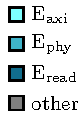
\includegraphics{assets/legend.pdf}
    }
    \hfill
    \subcaptionbox{PCM\label{fig:sunburst_avg_conf_proc_pcm}}{
        \import{assets/power_analysis}{pre}
\begin{tikzpicture}
    \pie[
        radius=2.3,
        text=pin,
        hide number,
    ]{
        1.2/1.2\%,
        2.6/2.6\%,
        5.0/5.0\%,
        3.0/3.0\%
    }
    \pie[
        radius=2.3,
        hide number,
        color={gray, bluehue2, bluehue4, bluehue6},
        before number=\printonlylargeenough{2},
        after number=\ifprintnumber\%\fi
    ]{
        1.2/,
        2.6/,
        5.0/,
        3.0/
    }
    \pie[
        radius=1.8,
        text=inside,
        color={blue!60, red!60},
    ]{
        11.8/$\econf$,
        88.2/$\eproc$
    }
\end{tikzpicture}

    }
    \caption{Average energy consumption distribution of the models listed in \cref{tab:example_models_stats}}
    \label{fig:example_models_avg_conf_proc}
\end{figure}
    